\paragraph{Lagrangian}
We have 6 degrees of freedom: $\vec{R}$, $\theta$, $\varphi$, $\psi$.
$$L = \frac{1}{2} M \vec{\dot{R}}^2 + \frac{1}{2} I_i \Omega_i^2 + U\left( \vec{R}, \theta, \varphi, \psi \right)$$
For $\vec{R}$:
$$\vec{\dot{P}}=M\vec{\ddot{R}} = -\vec{\nabla}_R U = \vec{F}$$
\paragraph{Movement equations from momentum and angular momentum}
$$\vec{\dot{P}} = \sum_i m_i \vec{v}_i = \sum_i \vec{f}_i = \vec{F}$$
For angular momentum:
$$\vec{\dot{M}} = \sum_i m_i \underbrace{\vec{\dot{r}}_i \times \vec{v}_i}_{0} + m_i \vec{r}_i \times \vec{\dot{v}}_i =  \sum_i m_i \vec{r}_i \times \vec{\dot{v}}_i =  \sum_i \vec{r}_i \times \vec{\dot{p}}_i = \vec{N}$$
$$\frac{d}{dt} \vec{M} = \vec{N}$$
$$\left[\frac{d}{dt} \vec{M}\right]_{\text{lab}} = \left[\frac{d}{dt} \vec{M}\right]_{\text{body}} + \vec{\Omega} \times \vec{M}$$
If we take inertial system such that a given moment axes are same as axes of body, after rotation, if $\vec{M}$ in body's FOR is unchanged, and thus is equal $\vec{\Omega}\times \vec{M}$.
$$\frac{d\vec{M}}{dt}_i = \dot{M}_i + \epsilon_{ijk} \Omega_j M_k = I_i \dot{\Omega}_i + \epsilon_{ijk} \Omega_j I_k \Omega_k = N_i$$
Then Euler equations are;
$$\begin{cases}
 I_1 \dot{\Omega}_1 + \Omega_2 \Omega_3 (I_3-I_2) = N_1\\
 I_2 \dot{\Omega}_2 + \Omega_1 \Omega_3 (I_1-I_3) = N_2\\
 I_3 \dot{\Omega}_3 + \Omega_1 \Omega_2 (I_2-I_1) = N_3\\
\end{cases}$$

\paragraph{Example}
Symmetric gyroscope: in body's system $\vec{N} = 0$, then
$$\begin{cases}
I_1 \dot{\Omega}_1 + \Omega_2 \Omega_3 (I_3-I_1) = 0\\
I_1 \dot{\Omega}_2 + \Omega_1 \Omega_3 (I_1-I_3) = 0\\
I_3 \dot{\Omega}_3  = 0\\
\end{cases}$$
We can easily see that
$\Omega_3 = \frac{M_3}{I_3}$. Define
$$\omega = \Omega_3 \frac{I_1+I_3}{I_1}$$
Then
$$\begin{cases}
\dot{\Omega}_1 = -\omega \Omega_2\\
\dot{\Omega}_2 = -\omega \Omega_1\\
\end{cases}$$
Differentiating:
$$\begin{cases}
\ddot{\Omega}_1 = -\omega^2 \Omega_2\\
\ddot{\Omega}_2 = -\omega^2 \Omega_1\\
\end{cases}$$
Then
$$\begin{cases}
\Omega_1  =  A \cos \left( \omega t+ \Psi_0  \right)\\
\Omega_2  =   A \sin \left( \omega t+ \Psi_0  \right)\\
\Omega_3  =  \frac{M_3}{I_3}\\
\end{cases}$$

The symmetry axis is making circular motion around vertical axis. Lets find precession frequency:
$$\omega_{pr} = \frac{V}{R} = \frac{\Omega_1R_3}{R_3 \sin \theta}  = \frac{\Omega_1}{\sin \theta}  = \frac{\Omega_1I_1}{I_1\sin \theta} = \frac{M_1}{I_1\sin \theta} = \frac{M\sin \theta}{I_1\sin \theta} = \frac{M}{I_1}$$
\paragraph{Assymetric gyroscope}
$\vec{N}= 0$ and $I_1 < I_2 < I_3$. From conservations:
$$E = \frac{1}{2} \left( I_1\Omega_1^2 + I_2 \Omega_2^2 + I_3\Omega_3^2 \right) = \text{const}$$
$$m^2 = M_1^2+M_2^2+M_3^2 = \text{const}$$
Then
$$\frac{M_1^2}{2EI_1}+\frac{M_2^2}{2EI_2}+\frac{M_3^2}{2EI_3} = 1$$

The body trajectory moves on intersection of ellipsoid and sphere:
\begin{center}
	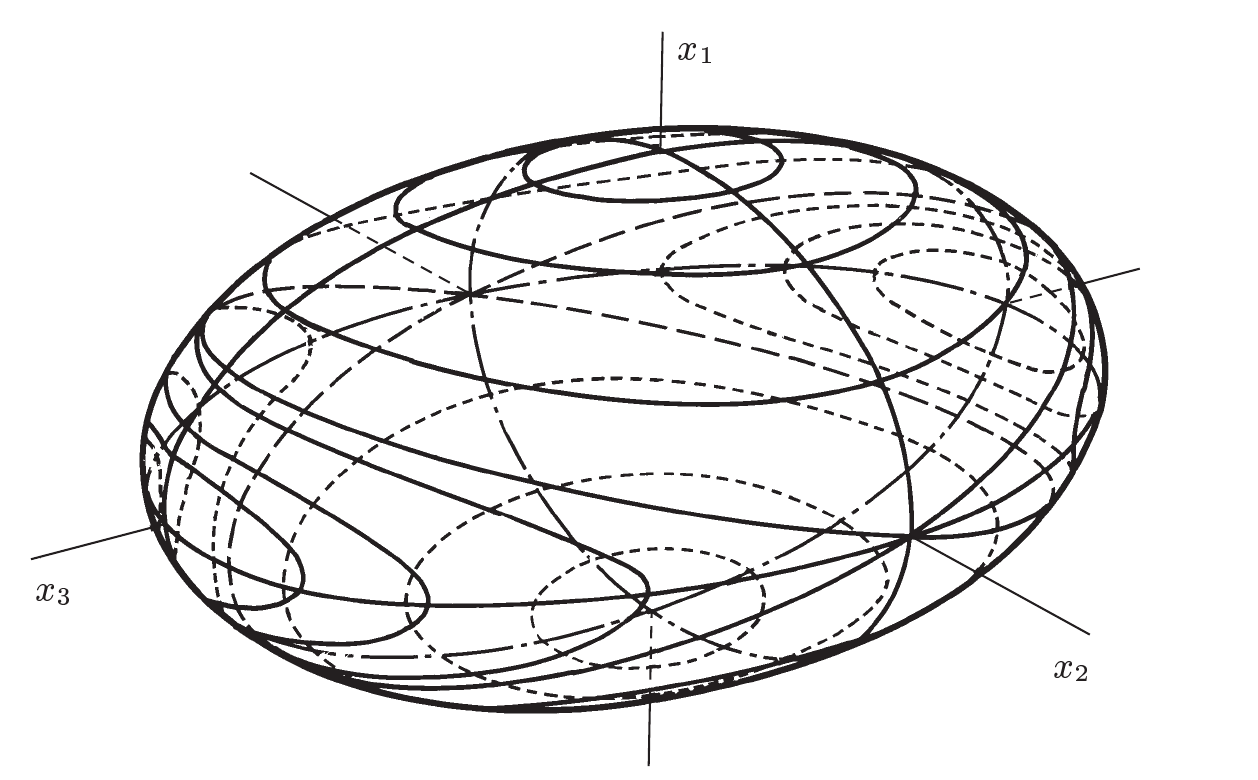
\includegraphics[width=\linewidth]{./lect23/1.png}
\end{center}
Those are intersections of ellipsoid and spheres of different radii.

If we denote 
$$\begin{cases}
\alpha_1 = -\frac{I_3-I_2}{I_1} < 0\\
\alpha_2 = -\frac{I_1-I_3}{I_2} > 0\\
\alpha_3 = -\frac{I_2-I_1}{I_3} < 0
\end{cases}$$
Suppose rotation close to one of the axis:
$$\begin{cases}
\Omega_1 = \omega_1\\
\Omega_2 = \Delta\omega_2\\
\Omega_3 =  \Delta\omega_3\\
\end{cases} \quad \Delta \omega_2, \Delta \omega_3 \ll \omega$$
Then Euler equations are:
$$\begin{cases}
\dot{\omega} = \Omega_1\Omega_2\alpha_3 = 0\\
\Delta \dot{\omega}_1 =\omega \Delta \omega_2 \alpha_1\\
\Delta \dot{\omega}_2  =\omega \Delta \omega_1 \alpha_2\\
\end{cases}$$
Thus
$$\Delta \ddot{\omega}_1 = \omega^2 \alpha_1 \alpha_2 \Delta \omega_1 \omega = \text{const}$$
and depending on positive or negative coefficient 
